% 
% ======================================================================
\RequirePackage{docswitch}
% \flag is set by the user, through the makefile:
%    make note
%    make apj
% etc.
\setjournal{\flag}

\documentclass[\docopts]{\docclass}

% You could also define the document class directly
%\documentclass[]{emulateapj}

% Custom commands from LSST DESC, see texmf/styles/lsstdesc_macros.sty
\usepackage{lsstdesc_macros}

\usepackage{graphicx}
\graphicspath{{./}{./figures/}}
\bibliographystyle{apj}

% Add your own macros here:

\newcommand{\Mcal}{\texttt{Metacalibration}}
\newcommand{\mcal}{\texttt{metacalibration}}
\newcommand{\snr}{S/N}


% 
% ======================================================================

\begin{document}

\title{ Problems and Solutions for LSST Shape Measurement }

\maketitlepre

\begin{abstract}

LSST weak lensing science has unprecedented requirements for the modelling of the LSST point spread function and the accurate measurement of galaxy shapes in the face of blending. In this document, we describe the results of a workshop on these issues held at Point Montara in February 2017. We discuss available solutions for the PSF modelling and shape measurement, lessons learned from their use in the Dark Energy Survey, remaining open issues, and progress and plans towards fixing those. In addition, we lay out a strategy for handling multi-epoch image data in an API useful with present weak lensing image analysis codes and a framework for validating PSF and shape measurement through image simulations.

\end{abstract}

% Keywords are ignored in the LSST DESC Note style:
\dockeys{latex: templates, papers: awesome}

\maketitlepost

% ----------------------------------------------------------------------
% 

\section{Introduction}
\label{sec:intro}

\FIXME{We skip the introduction for now, but keep an introduction to this \LaTeX\xspace class for reference.}

This is a paper and note template for the LSST DESC \citep{Overview,ScienceBook,WhitePaper}.
You can delete all this tutorial text whenever you like.

You can easily switch between various \LaTeX\xspace styles for internal notes and peer reviewed journals.
Documents can be compiled using the provided \code{Makefile}.
The command \code{make} with no arguments compiles \code{main.tex} using the  \code{lsstdescnote.cls} style.
If you want to upgrade your Note into a journal article, just choose a journal name, between \code{make apj} (ApJ preprint format), \code{make apjl} (which uses the \code{emulateapj} style), \code{make prd}, \code{make prl}, and \code{make mnras}.


There are a number of useful \LaTeX\xspace commands predefined in \code{macros.tex}.
Notice that the section labels are prefixed with \code{sec:} to allow the use of the \verb=\secref= command to reference a section (\ie, \secref{intro}).
Figures can be referenced with the \verb=\figref= command, which assumes that the figure label is prefixed with \code{fig:}.
In \figref{example} we show an example figure.
You'll notice that the actual figure file is found in the \code{figures} directory.
However, because we have specified this directory in our \verb=\graphicspath= we do not need to explicitly specify the path to the image.

The \code{macros.tex} package also contains some conventional scientific units like \angstrom, \GeV, \Msun, etc. and some editorial tools for highlighting \FIXME{issues}, \CHECK{text to be checked}, \COMMENT{comments}, and \NEW{new additions}.


Similar to the figure before, here we have included a table of data from \code{tables/table.tex}.
Notice that again we are able to reference \tabref{example} with the \verb=\tabref= command using the \code{tab:} prefix.
Also notice that we haven't needed to specify the full path to the table because in the \code{Makefile} we include \code{./tables} directory in the \code{\$TEXINPUTS} environment variable.

\input{table}

Equations appear as follows, and can be referred to as, for example, \eqnref{example} -- just as for tables, we use the \verb=\eqnref= command using the \code{eqn:} prefix.
\begin{equation}
  \label{eqn:example}
  \langle f(k) \rangle = \frac{ \sum_{t=0}^{N}f(t,k) }{N}
\end{equation}


\figref{example} shows an example figure, referred to with the \verb=\figref= command and the \code{fig:} prefix.

\begin{figure}
\includegraphics[width=0.9\columnwidth]{example.png}
\caption{An example figure: the LSST DESC logo, copied from \code{.logos/desc-logo.png} into \code{figures/example.png}. \label{fig:example}}
\end{figure}

If you are planning on committing your paper to GitHub, it's a good idea to write your tex as one sentence per line.
This allows for an easier \code{diff} of changes.
It also makes sense to think of latex as \emph{code}, and sentences as logical statements, occupying one line each.
Each line must ``compile'' in the mind of the reader.

% ----------------------------------------------------------------------

\section{MEDS: Multi-epoch data structures}

\FIXME{write why we need this: unified API for PSF modelling / shape measurement / photometry codes to access single frame image, weight, astrometry and PSF information}

\subsection{High-order instrumental astrometric distortions in MEDS}

\FIXME{Gary, Troxel, Mike, Erin: describe how this is implemented}

The \textsc{meds} python class would allow for flexibly swapping out the WCS in the input file FITS header by something more elaborate if we have the base class provide access functions for the \texttt{cutout\_row/col} variables (in addition to the Jacobian) \FIXME{(Erin)}. A derived class could then implement these differently, e.g. by evaluating Gary's WCS \FIXME{(Gary)}. Both this and the way shape measurement codes find the matching PSFEx model files could be implemented by an external simple table that maps exposure and CCD IDs to auxiliary filenames.


\subsection{A MEDS API for LSST}

\FIXME{Jim, Erin, Joe, Josh, Daniel: describe how this is implemented; it seems like an API that generates an object's MEDS information on the fly could be feasible}

% ----------------------------------------------------------------------

\section{PIFF: PSFs in the Full FOV}

\FIXME{write an introduction of why we need this: astrometric distortions -> WCS, coherent patterns over full FOV, Zernickes, better interpolation schemes}

\subsection{Gaussian Process Interpolation}

\FIXME{Josh, Gary, Mike, Niall, Pierre-Francois, Ami: describe}

\subsection{Errors on Adaptive Moments}

The wavefront-based PSF performs a $\chi^2$ fit to the adaptive moments of stars.  However, up to now we have not included an error on the adaptive moments in the fit.  We calculated the errors on the adaptive moments, using the following expressions from simple error propagation:
$$  \sigma^2(e_0) = \sum \left\{ \left[ (u-u_0)^2 + (v-v_0)^2  \right] K(u,v) \right\}^2 \sigma_{I}^2(u,v) $$
$$  \sigma^2(e_1) = \sum \left\{ \left[ (u-u_0)^2 - (v-v_0)^2  \right] K(u,v) \right\}^2 \sigma_{I}^2(u,v) $$
$$  \sigma^2(e_2) = \sum \left\{ \left[ (u-u_0)  (v-v_0)  \right] K(u,v) \right\}^2 \sigma_{I}^2(u,v) $$
where $\sigma_{I}(u,v)$ is the shot noise on an individual pixel and $K(u,v)$ is the kernel used by the HSM algorithm. Note that we have not yet included a contribution from the error on the centroids, nor from the (omitted) normalization term. 

To test this calculation, we used an ensemble of simulated stars, constructed with arbitrary aberration, and with shot noise appropriate for different choices of star S/N. For a stellar flux of $10^5$ photo-electrons, we created 5000 noisy stars, calculated their adaptive moments and errors, and plot the pull distribution for $e_0$, $e_1$ and $e_2$ (note that our $e_1$ and $e_2$ are unnormalized) in Figure~\ref{fig:momerror}.  The pull distributions have RMS  somewhat larger than 1., and we find very similar RMS values independent of flux for values from $10^6$ down to $4\times10^3$.  We suspect that the errors are underestimated because we omit the contribution to the error from the uncertainty in the centroids and the normalization.  


\begin{figure}[h]
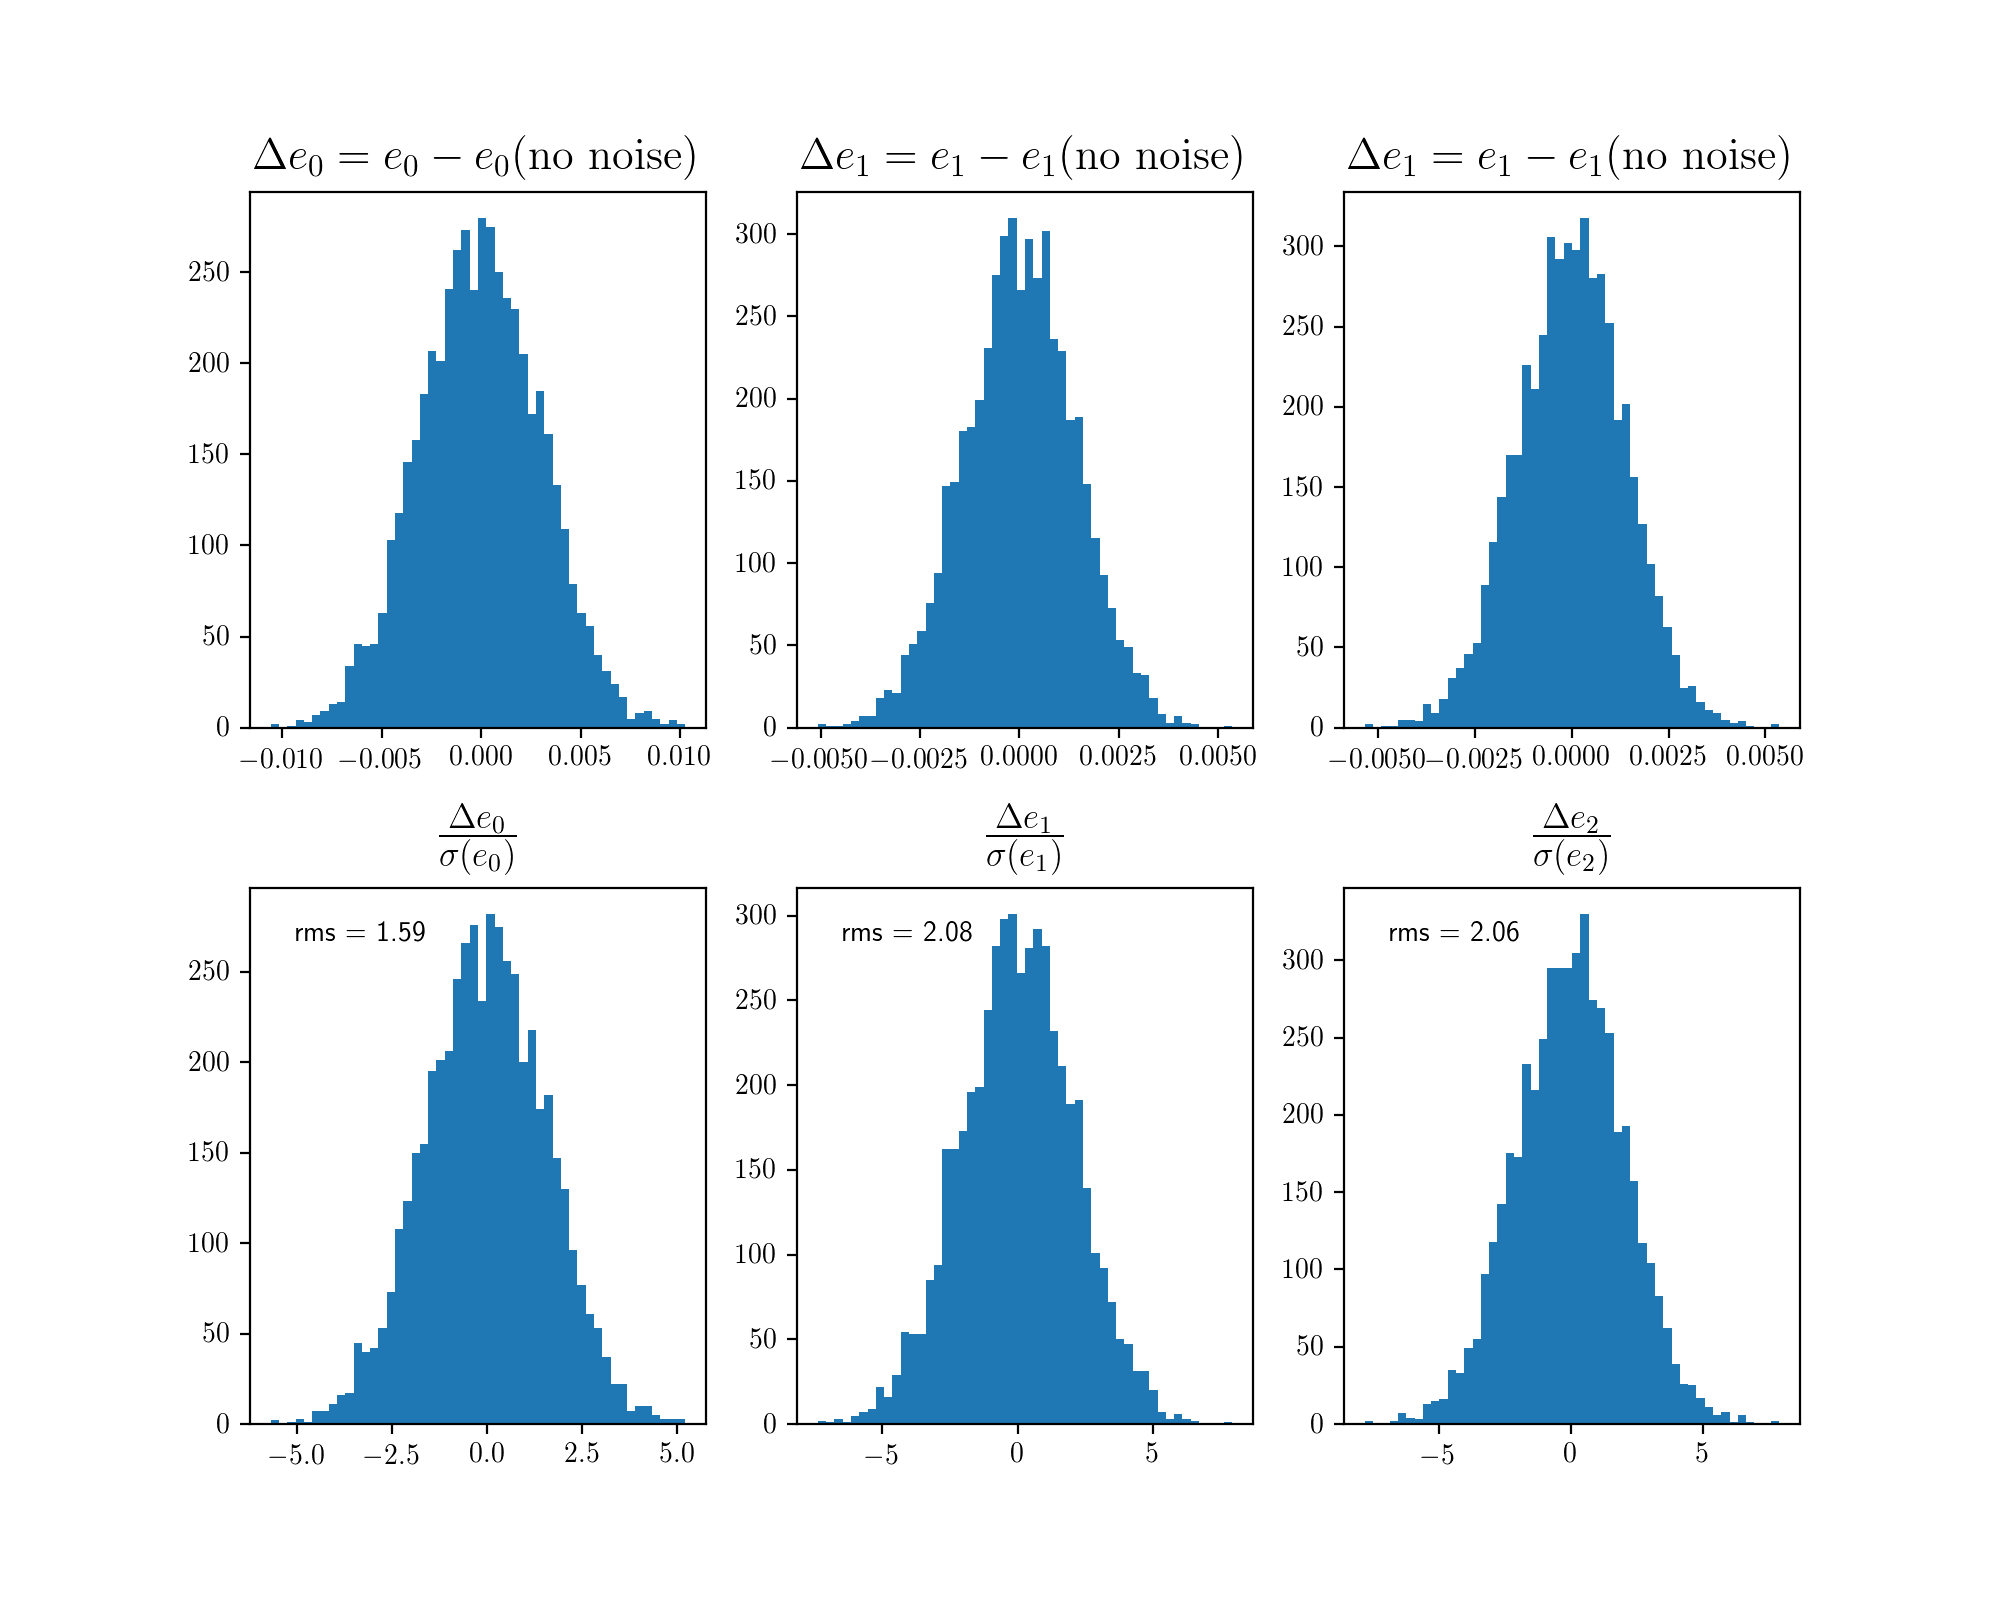
\includegraphics[width=0.9\columnwidth]{moment-errors-flux1e5.png}
\caption{The pull distributions for $e_0$, $e_1$ and $e_2$ from a sample of simulated stars with $S/N = 316$. The errors are underestimated by a factor which is independent of S/N. \label{fig:momerror}}
\end{figure}

\subsection{Combining PSF Models}

A goal with PIFF is to model the PSF as a combination of the optical and atmospheric PSFs.
Because these two PSFs have significant differences in implementation, they need to be combined together within PIFF.
Chris wrote a new \texttt{PSF} class, \texttt{CompoundPSF}, while at the lighthouse.
This class can take an arbitrary number of PSFs, and fits each piece iteratively.
The final PSF is a convolution of the PSFs.

\section{Shape measurement}

\FIXME{quick intro of lessons learned from DES Y1}

\subsection{BFD on real data}

\FIXME{Gary, Daniel, Joe, Katie, Ami: describe}

The two components missing for this are
\begin{itemize}
\item a variant of \texttt{simpleImage} (see \texttt{momentcalc.py} in the BFD repository) that can take multiple postage stamps of the same galaxies with their respective WCS registrations (in the form of the position of a centroid estimated in WCS and transformed to the postage stamp pixel system) and Jacobians, PSF models, and an estimate of the overall centroid in WCS \FIXME{(Katie)}
\item a function that can get these inputs to the new variant of \texttt{simpleImage} from a MEDS file (using the python \texttt{meds} or a derived class) \FIXME{(Daniel)}
\end{itemize}


% ----------------------------------------------------------------------

\section{An image simulation pipeline for PSF and shape measurement validation}

\FIXME{Joe, Mike, Erin, Troxel, Gary, Daniel, Niall, Ami, Katie: describe}

\subsection{Goals}
Goals: Simulation engines primarily for validation. Win some Gin from Catherine Heymans.

The subsections below describe stages of this process and the options or considerations for it.

\subsection{(Statistical) Requirements}

It's important to define cosmology-driven requirements for the simulation, as these will set the simulation volume requirements and thus the computing requirements etc.. Particularly important to do this if we e.g. need to find/apply for more computing resources.

I've brain-dumped a few thoughts on a couple of different (but certainly related) approaches we could take to this, (i) how many galaxies/galaxy pairs do we need to test our desired statistics to a given precision? (ii) How many realisations of our survey do we need test our desired statistics to a given precision? I think the second approach is probably simpler because a simulation of our survey will automatically (of course limited by the simulation realism) have distributions of certain relevant survey properties (e.g. noise, PSF) that match the real data. 

We want to demonstrate that our shear estimation pipelines can recover unbiased shear-shear and tangential shear signals to better than $X_i\%$, $Y_i\%$  for in $n_z$ redshift bins, $i$, for $0<z<z_{\mathrm{max}}$ for some range of scales $\theta_{\mathrm{min}} < \theta < \theta_{\mathrm{max}}$ (we could also phrase in terms of $l$ and $C_l$. This requires:
\begin{align}
\left<(1+m_i)(1+m_j)\right>(\theta) + \left<c_i c_j\right>(\theta)/\left<\gamma \gamma\right>(\theta) < X\%, \\ 
\left<n_{\mathrm{lens}}(1+m_i)\right> < Y\%.
\end{align}

Ignoring the scale dependence, assuming a constant shear, and that we calculate $m$ as
\begin{equation}
\left<m_i\right> = \left<\frac{\gamma_{\mathrm{obs}}-\gamma_{\mathrm{true}}}{\gamma_{\mathrm{true}}}\right>,
\end{equation}
where the (possibly weighed) averaging is over all galaxies in redshift bin $i$.
\begin{equation}
\sigma_m = \frac{\sigma_e}{\gamma_{\mathrm{true}} \sqrt{N_{\mathrm{gal}}}}
\end{equation}
We want e.g. $\sigma_{m_i} < 0.5 X_i\%$, so e.g. for $X_i = 1\%$, $\gamma_{\mathrm{true}}=0.01$, $\sigma_e = 0.2$, we'd need to simulate $1.6\times10^7$ galaxies per redshift bin.

Are we worried about scale dependence? For shear-shear, we get selection biases due to blending (blended galaxies are more likely to be in high galaxy number density, high convergence regions \citep{hartlap2011,maccrann2017}). Spatial correlations in observing conditions may produce spatial correlations in the shear biases. For tangential shear, increased crowding closer to clusters/lens galaxies will produce scale dependent shear biases \citep{melchior2015,simet2015}.

An alternative way to think about the requirements is to first assume that we want to simulated $N_{\mathrm{sim}}$ copies of our survey ($N_{\mathrm{sim}}$ could, but probably wouldn't be less than 1). This approach has the advantage that (to the extent that the simulated survey properties are realistic), the simulated survey properties (e.g. noise, PSF etc.) will have the same distributions as the data. If we want to know the accuracy to which our pipeline recovers some statistic  to better than a fraction $f$ of the shape noise errors on that statistic we have in the real data, then we require $N_{\mathrm{sim}} = 1/f^2$ realisations of our data. 

Discussion points:
\begin{itemize}
\item{What should $f$ be? Note that most of the statistics we use are cosmic variance limited on large scales, so beating down the shape noise may not be so relevant. We will know the `cosmic variance' (or rather we'll know the particular realisation of the cosmological signal) in the simulation.}
\item{How can we reduce $N_{\mathrm{sim}}$? Boost the shear signal - the stronger the simulate signal, the better fractional accuracy can be achieved. However, concerns exist about higher order shear biases, and breaking the relations between galaxy number density and shear. For postage-stamp styles simulations, presumable we can use ring-test type tricks to reduce shape noise. Is there something similar we can use for the detection simulation?}
\item{What kind of shear fields should we use? If we use something realistic (e.g. from ray-tracing), how do we test that we're recovering it correctly, given that a given method will only use a subset of the galaxies...}
\end{itemize}

We envisage two main modes of the image simulations. 
\begin{enumerate}
\item \emph{Tide-pool} Fast, straight to postage-stamps simulations where different marine organisms (e.g. complex morphology, PSF model errors) are turned on and off. Galaxies written straight to MEDS files, or are generated on-the-fly. No neighbours.
\item \emph{Pacific} Full single-epoch survey images are rendered. Coadd images are produced for detection/deblending. PSF estimation is performed on the SE images. MEDS files produced using SE images and coadd information. Some shortcuts probably needed!
\end{enumerate}

Three main initial tasks:
\begin{enumerate}
\item{Finish writing up this plan (NM+)}
\item{Design and write simulation software framework (JZ+)}
\item{Design and write input galaxy catalog 
$->$ galaxy appearance module}
\item{Estimate timings + memory usage for simulation steps. Could split this into several tasks e.g. image rendering timing (i.e. mostly GalSim stuff) (MJ+?), coadding+detection (i.e. SWARP + SExtractor) timing.}
\item{Estimate computing requirements for various sims modes.}
\end{enumerate}

\subsection{Required Ingredients}

\subsubsection{Input Catalogues}

Requirement: Galaxy sample with physically sensible clustering, redshift evolution, morphologies, colours, and correlations between the above. Sufficiently complex morphologies to test model bias, and sensible variation in morphology between filters. 

\begin{itemize}
\item Starting from an observed catalog is problematic: measured quantities get noisy at the faint end, we won't get sub-detection objects.
\item Proposal: Start from N-body + galaxy simulation e.g. BCC.
\item Map simulation outputs (e.g. color, size) to image properties in each filter (e.g. bulge/disc, size, amount of star formation knots). Look into Lanusse method.
\item Needs to go to high enough redshift and depth for deep fields (and for sufficient sub-detection objects in wide-field).
\end{itemize}

\subsubsection{Shear Field}

The following options, probably we'll want to do one of the first two for the Pacific simulation. Other options fine for tide-pool simulation. 
\begin{itemize}
\item From saved N-body results (see above)
\item Spatially varying but without evolution within a redshift bin
\item Spatially varying but without redshift evolution
\item Constant
\end{itemize}

\subsubsection{Survey Details}

\begin{itemize}
\item Real data pointings
\item Exposure times - from real survey
\item Noise levels - from real survey
\item Sky background - from real survey
\item Deep data - Same process but with more exposures
\end{itemize}


\subsubsection{True Astrometry}

\begin{itemize}
\item Flat WCS
\item Real image WCS
\item Gary's WCS
\item FITS header WCS
\item One of the above + some error distribution
\end{itemize}

\subsubsection{True PSF}

\begin{itemize}
\item Estimated real ones from Piff
\item Additional complexity, adding variation on smaller scales than 
\item Fixed values
\item Colour-dependence of PSF.
	  Full implementation 100 times slower.
	  Could make it a function of a single colour parameter, linearly interpolated.
	  Effective PSF from real SED? Function of (g-i).
	  Intra-band resolution of PSF.  Do this at n wavelengths.
	  Like using a chunky SED.
\end{itemize}

\subsubsection{Star Catalogue}

\begin{itemize}
\item Gaia?
\item Randomly, function of latitude.
\item SEDs - some in galsim already, need more?
\end{itemize}

\subsubsection{Artifacts}
\begin{itemize}
\item Tape bumps
\item CTI
\item Brighter-fatter
\item Non-linearity
\item Non-convolutional things
\item Image artifacts
\end{itemize}

\subsubsection{Masking}

\begin{itemize}
\item Real
\item Real + artifacts
\end{itemize}

\subsubsection{Single-epoch Rendering}

\begin{itemize}
\item GalSim
\end{itemize}

\subsubsection{Coadding}
\begin{itemize}
\item Run full pipeline - i.e. run swarp
\item Shortcut option: draw coadd directly. What does this miss? What is required to test this?
\end{itemize}

\subsubsection{Detection \& Segmenting}
\begin{itemize}
\item Needed for lists of detected objects and segmentation masks
\item Run full pipeline - SExtractor on coadd
\item Generate object list and seg map from truth catalogs
\end{itemize}

\subsubsection{Estimated PSF}
\begin{itemize}
\item Find starting stars - on coadd using SExtractor? Can we do this without spread-model?
\item Run PIFF
\item Use truth
\end{itemize}

\subsubsection{Estimated astrometry}
\begin{itemize}
\item Cannot re-do the actual astrometry process
\item Use the original FITS ones
\item Use truth + some error term
\end{itemize}

\subsubsection{Photometric Calibration}
\begin{itemize}
\item Could place a small error on the truth - scale objects by some factor.
\end{itemize}

\subsubsection{MEDS}
\begin{itemize}
\item Make a MEDS file and run on it!
\end{itemize}



\section{\Mcal\ Response for Stars}

Testing to see if we can cause positive responses for stars in a simulation.
In some scenarios we see $<R> \sim 0.25$ in real data.

\subsection{Variations in PSF}

Consider the case where the PSF model used is accurate in the mean but 
for an individual galaxy the truth varies significantly.  The response
for stars at high \snr ($> 100$), and using forward modeling, is shown in
figure \ref{fig:Rstarfm}.  The same for adaptive moments, without
PSF correction. The response has mean about 0.1 for forward modeling,
but nearly zero for adaptive moments.  In both cases the distribution
is nearly gaussian, whereas in real data it tends to be highly asymmetric,
with mode at $R \sim 0.5$.


\begin{figure}[p]
    \centering
    \includegraphics[width=0.5\textwidth]{figures/test_psf_var-000-R11.pdf}

    \caption{Response for high \snr\ stars when varying the PSF from
    object to object, but using
    the mean model when performing \mcal\ operatioins, using the forward modeling estimator.
    Parameters of the best fit gaussian are shown. }

	\label{fig:Rstarfm}

\end{figure}
\begin{figure}[p]
    \centering
    \includegraphics[width=0.5\textwidth]{figures/test_psf_var-000-R11-admom.pdf}

    \caption{Same as figure \ref{fig:Rstarfm}, but adaptive moments estimator with no PSF correction}

	\label{fig:Rstaram}

\end{figure}



% ----------------------------------------------------------------------

\subsection*{Acknowledgments}

We acknowledge financial and organizational support for our workshop from LSSTC and KIPAC and the hospitality of Hostelling International.

\input{acknowledgments}

%{\it Facilities:} \facility{LSST}

% Include both collaboration papers and external citations:
\bibliography{lsstdesc,main}

\end{document}
% ======================================================================
% 
